\chapter{Implementation}

This project is implemented in PHP 5, which can be run in a web browser. The decision to create the thesis on a browser system was made because users do not have to install any software on their machines and it reduces the time to solve a task. Furthermore, it also allows to make changes to the code without a need for users to re-download it.
Finally, PHP is chosen because of his ability to access the UNIX command line tools, which are needed in this project and because of its big community.
\newline

The software runs on an Ubuntu server distribution with version 14.04, which has a MySQL database installed. This choice has been made because one can access the distribution and install some frameworks as FFmpeg, Cron and Octave.
\newline

To display the video to the users, the HTML5 video element is used, with the controls disabled. The time display video could be set with JavaScript. This has the advantage that the whole video file does not need to be loaded. Getting the current time of the video enables storing the events' temporal information in the database.
\newline

Because PHP is inappropriate to perform matrix calculations, a Matlab script is used to calculate the new bases of the points described in Section \ref{sec:Dist_calc}. The Matlab scripts run from the PHP command line framework using Octave \cite{Eaton:2002}, an interpreter language for numerical calculations.



\paragraph{Events}

To remove the tasks that have been started and not finished, and are stored in the table of the database system, the MySQL Event Scheduler \cite{MySQL:Events} is used.
This event checks every 20 minutes if events older than half an hour exist on database entity holding the tasks started but not finished. If there are some, they will be deleted by the Event Scheduler, which frees up the tasks again for users.



\paragraph{Image handling}

To create the images for the video player extension, FFmpeg \cite{FFMPEG:1} is used, which is an open source Linux-based multimedia framework able to manipulate multimedia data. This distribution allows creating images of a video file at a specified sequence and in a specified interval.

With FFmpeg, different variables are set as the start and end times of the sequence where FFmpeg should generate images. There is also a variable to set the interval in which the frames should be created, and by setting the images to a smaller size than the videos size the storage space can be reduced.
For the purposes of this project, the image size is set to 12 KB.
\newline

To store the images created for every task and time, a new folder is used with the token as the name. Taking the token as the folder name ensures that all folder names are unique and the right images can be selected for every task.

To prevent the file system from overloading, Cron \cite{Keller:1999} is used, which allows one to call a script every half hour, which deletes every folder older than one hour.

\paragraph{Microworkers}\label{sec:Microworkers}

For the experiments, an international campaign in the category “search, click and engage” has been created on Microworkers. In the first experiment, the estimated time to solve the task has been set to 10 minutes.


\begin{minipage}{\linewidth}
      \centering
      \begin{minipage}{0.45\linewidth}
          \begin{figure}[H]
              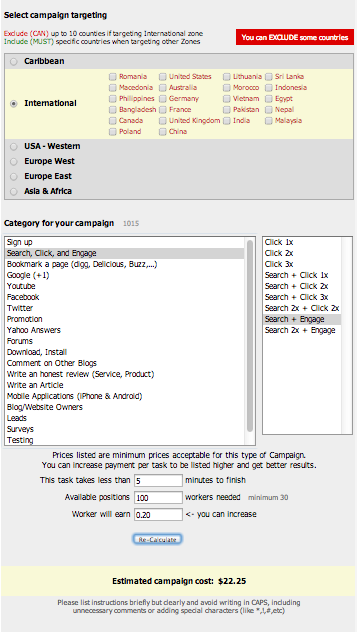
\includegraphics[width=\linewidth]{microworkers/Microworkers1}
              \caption{First part of Microworkers basic campaign settings}
              \label{fig:microworkers1}
          \end{figure}
      \end{minipage}
      \hspace{0.05\linewidth}
      \begin{minipage}{0.45\linewidth}
          \begin{figure}[H]
              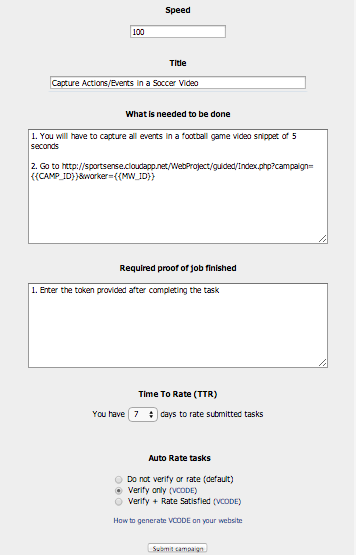
\includegraphics[width=\linewidth]{microworkers/Microworkers2}
              \caption{Second part of the Microworkers basic campaign settings}
              \label{fig:microworkers2}
          \end{figure}
      \end{minipage}
\end{minipage}
\newline

Figures \ref{fig:microworkers1} and \ref{fig:microworkers2} show how the campaign was created on Microworkers.
Based on the results of Google Analytics as shown in Section \ref{sec:analytics}, in the final experiments, the time workers need to finish a task was reduced to 5 minutes in further tests.


\paragraph{Interface server database}
To connect PHP with the database, PHP Data Objects \cite{PDO:1} is used.
PDO is an object-oriented interface between the database and PHP. The advantage of PDO is that it does not have to be rewritten to connect to another database engine. The only difference between the database systems is that the parameter that defines the driver must be changed when creating the instance of the constructor.
